\paragraph{La classe ConnectionCANdroid}

\begin{minipage}
    {\linewidth}
    \centering
    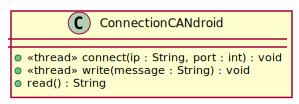
\includegraphics[width=0.5\linewidth]{../schemas/Conception_detaillee/classe_connectionCANdroid.pdf}
    \captionof{figure}{Diagramme de classe de ConnectionCANdroid}
\end{minipage}

\subparagraph{Philosophie de conception \newline} 

\medspace

La classe ConnectionCANdroid a pour rôle de se connecter au programme {\nomLogiciel}, d'envoyer des données et d'en lire. 

\subparagraph{Description structurelle \newline}

\medspace

\textbf{Attributs :}

N.A.

\textbf{Services offerts :}

\begin{itemize}
    \item \textbf{connect(ip : String, port : int) : void} --- Opération qui permet de se connecter au port et à l'IP donnés en paramètres. 
    \item \textbf{write(message : String) : void } --- Opération qui permet d'écrire sur le socket.  
    \item \textbf{read() : String } --- Opération qui permet de lire le socket.
\end{itemize}